\section{Experimental Setup}
\label{sec:setup}

The experimental setup considers a large image dataset, three state-of-the-art neural network models and two high-end platforms.
The following sections describe all theses elements in detail.

\subsection{Image Dataset}
We consider the ImageNet ILSVRC-2012 
dataset~\cite{imagenet}.
The original ImageNet dataset includes three sets of images of 1000 classes each:
training set (1.3 million images), validation set (50,000 images) and
testing set (100,000 images).
Considering 1000 classes makes the training process around 170 hours long, which is prohibitively expensive for large experimental campaign considering different network models, batch sizes and hardware platforms.
To reduce the execution time of our experiments we consider a subset of 200 
classes for both the training and the validation dataset, which keeps the training time under manageable margins.
%  To speedup our experiments without hampering
%the quality of the results, we select a same set of 200 classes for both the
%training set and the validation set as our dataset.
%For the rest of this paper, 
We refer to the 200 and 1000 classes datasets as ImageNet200 and ImageNet1000, respectively.
Since it is a common practice~\cite{vgg}, we evaluate the ability of a certain network in 
properly dealing with the ImageNet ILSVRC-2012 dataset in terms of the top-5 validation error computed over the validation set.

\subsection{DNN Models and Training Parameters}
We apply the AWP algorithm along with the ADT procedure on three state-of-the-art 
DNN models: a modified version of Alexnet~\cite{alexnet} with an extra fully-connected layer of size 4096, the configuration A of the VGG model~\cite{vgg} and the Resnet network~\cite{resnet}. 
All hidden layers are equipped with a Rectified Linear Units (ReLU)~\cite{alexnet}.
The exact configurations of the three neural networks are shown in Table~\ref{table:config}. 
The Alexnet model is composed of 5 convolutional layers and 4 fully-connected ones, VGG contains 8 convolutional layers and 3 fully-connected ones and Resnet is composed of 33 convolutional layers and a single fully-connected one.

% Please add the following required packages to your document preamble:
% \usepackage{multirow}
\begin{table}[]
\caption{Neural network configurations: The convolutional layer parameters are denoted 
as ``conv<receptive field size>-<number of channels>''. The ReLU activation 
    function is not shown for brevity. The building blocks of Resnet
    and the number of times they are applied are shown in a single cell.}
    \begin{tabular}{|P{2.5cm}|P{2.5cm}|P{2.5cm}|}
\hline
    \textbf{Alexnet} & \textbf{VGG}  & \textbf{Resnet-34}  \\ \hline
\multicolumn{3}{|c|}{input(224x224 RGB image)}                                                                                                                                                 \\ \hline
conv11-64                                                  & conv3-64                                                      & conv7-64                                                           \\ \hline
\multicolumn{3}{|c|}{maxpool}                                                                                                                                                                  \\ \hline
conv5-192                                                 & conv3-128                                                     & \begin{tabular}[c]{@{}c@{}}conv3-64\\ conv3-64\\ x3\end{tabular}   \\ \hline
\multicolumn{2}{|c|}{maxpool}                                                                                             &                                                                    \\ \hline
conv3-384                                                 & \begin{tabular}[c]{@{}c@{}}conv3-256\\ conv3-256\end{tabular} & \begin{tabular}[c]{@{}c@{}}conv3-128\\ conv3-128\\ x4\end{tabular} \\ \hline
\multicolumn{2}{|c|}{maxpool}                                                                                             &                                                                    \\ \hline
conv3-384                                                  & \begin{tabular}[c]{@{}c@{}}conv3-512\\ conv3-512\end{tabular} & \begin{tabular}[c]{@{}c@{}}conv3-256\\ conv3-256\\ x6\end{tabular} \\ \hline
\multicolumn{2}{|c|}{maxpool}                                                                                             &                                                                    \\ \hline
conv3-256                                                 & \begin{tabular}[c]{@{}c@{}}conv3-512\\ conv3-512\end{tabular} & \begin{tabular}[c]{@{}c@{}}conv3-512\\ conv3-512\\ x3\end{tabular} \\ \hline
\multicolumn{2}{|c|}{maxpool}                                                                                             & avgpool                                                            \\ \hline
\multicolumn{2}{|c|}{FC-4096}                                                                                             & \multicolumn{1}{l|}{\multirow{2}{*}{}}                             \\ \cline{1-2}
\begin{tabular}[c]{@{}c@{}}FC-4096\\ FC-4096\end{tabular} & \multicolumn{1}{c|}{FC-4096}                                  & \multicolumn{1}{l|}{}                                              \\ \hline
\multicolumn{3}{|c|}{FC-200}                                                                                                                                                                   \\ \hline
\multicolumn{3}{|c|}{softmax}                                                                                                                                                                  \\ \hline
\end{tabular}
\label{table:config}
\end{table}

%\begin{table}
%\caption{Neural network configurations: The convolutional layer parameters are denoted 
%as ``conv<receptive field size>-<number of channels>''. The ReLU activation 
%function is not shown for brevity.}
%%\fontsize{3}{3}\selectfont
%%\resizebox{.45\textwidth}{!}{
%\end{tabular}
%%}
%%\vspace{0.2cm}
%\label{table:config}
%%\vspace{-0.5cm}
%\end{table}


We use momentum SGD~\cite{momentum} to guide the training process with 
momentum set to 0.9. 
The training process is regularized by weight decay and  the $L_{2}$ 
penalty multiplier is set to $5\times10^{-4}$. 
We apply a dropout 
regularization value of 0.5 to fully-connected layers.
We initialize the weights using a zero-mean normal distribution 
with variance $10^{-2}$. 
The biases are initialized to $0.1$ for Alexnet and $0$ for both VGG and Resnet networks.
For the Alexnet and VGG models we consider training batch sizes of 64, 32 and 16.
To train the largest network we consider, Resnet, we consider batch sizes of 128, 64 and 32.
The 16 batch size incurs in a prohibitively expensive training process for Resnet and, therefore, we do not use it in our experimental campaign. 
%
%There are several factors to take into consideration that affect the
%benefits provided by this papers' proposals.
%Among the most important ones we have the number of weights of the considered neural network, 
%which define the size of the data transfers over which our solution is deployed, 
%or the batch size, which defines the number of samples each batch is composed of. 
%Since the network weights are updated every time a batch is processed, the smaller 
%the batch size is, the more frequent are the weight updates and, thus, the larger 
%is the potential of our solution for improving performance.
%In order to cover these factors,
%we train both neural networks using a set of three batch sizes: 64, 32 and 16.
%

For Alexnet we set the initial learning rate to $10^{-2}$ for the 64 batch size and decrease it by factors of 2 and 4 for the 32 and 16 batch sizes, respectively.
In the case of VGG we 
set the initial learning rate to $10^{-2}$ for the 64, 32 and 16 batch sizes, as in the state-of-the-art~\cite{vgg}.  
In the case of Resnet the learning rate is $10^{-2}$ for the 
batch size of 32 and 0.1 for the rest. 
For all network models we apply exponential decay to the learning rate throughout the whole training process in a way the learning rate decays every 30 batches by a factor of 0.16, as previous work suggests~\cite{alexnet2}.
For Resnet we obtain better results by adapting precision at the Resnet building blocks level~\cite{resnet} instead of doing so in a per-layer basis.
%\textcolor{cyan}{Our preliminary experiments suggest that by applying our approach 
%to all of the layers separately on Resnet does not provide any benefit. Instead, 
%we group the layer in terms of the resnet building blocks~\cite{resnet} and apply our approach on 
%that level.}

\subsection{Implementation}
Our code is written in Python on top of Google Tensorflow~\cite{tensorflow}.
Tensorflow is a data-flow and graph-based numerical library where 
the actual computation is carried out according to a computational graph 
constructed beforehand.
The computational graph defines the order and the type of computations that are 
going to take place. It supports NVIDIA's NCCL library.

To enable the use of both Bitpack and Bitunpack routines, we integrate them into Tensorflow using its C++ API.
Tensorflow executes the two routines before sending 
the weights from the CPU to the GPU and right after receiving the weights on the 
GPU side, respectively.
The Bitpack routine is implemented using the OpenMP 4.0 programming model. 
There are two versions of this routine using either Intel's AVX2 or AltiVec instructions, as explained in Section~\ref{sec:approx}.
Bitunpack is implemented using CUDA 8.0 and CUDA 10.0 respectively on the two 
platforms~\cite{cuda}.

\subsection{Hardware Platforms}
\label{sec:platform}
We conduct our experiments on two clusters featuring the x86 and POWER architectures.
The x86 machine is composed of two 8-core Intel Xeon
\textregistered E5-2630 v3 (Haswell) at 2.4 GHz and a 20 MB L3 shared cache memory each. 
It is also equipped with two Nvidia Tesla K80 accelerators, each of which hosts two 
Tesla GK210 GPUs.
It has 128 GB of main memory, distributed in 8 DIMMs of 16 GB DDR4 @ 2133 MHz.
The 16-core CPU and the four GPUs are connected via a PCIe 3.0 x8 8GT/s.
The operating system is RedHat Linux 6.7.
Overall, the peak performance of the two 8-core sockets plus the four Tesla GK210 GPUs is 6.44 TFlop/s.

The POWER machine is composed of two 20-core IBM POWER9 8335-GTG at 3.00 GHz.  
It contains four NVIDIA Volta V100 GPUs. 
Each node has 512 GB of main memory, distributed in 16 DIMMS of 32 GB @ 2666 MHz.
The GPUs are connected to the CPU devices via a NVIDIA NVLink 2.0 interconnection~\cite{nvlink}.
The operating system is RedHat Linux 7.4.
The peak performance of the two 20-core sockets plus the four V100 GPUs is 28.85 TFlop/s.

%\begin{figure*}[!bhtp]
%        \centerline{
%            \includegraphics[scale=0.24]{figs/alex/small_3/alexnet_validation_top5_32-$A^2$DtWp.pdf}
%            \includegraphics[scale=0.24]{figs/alex/small_3/alexnet_validation_top5_16-$A^2$DtWp.pdf}
%            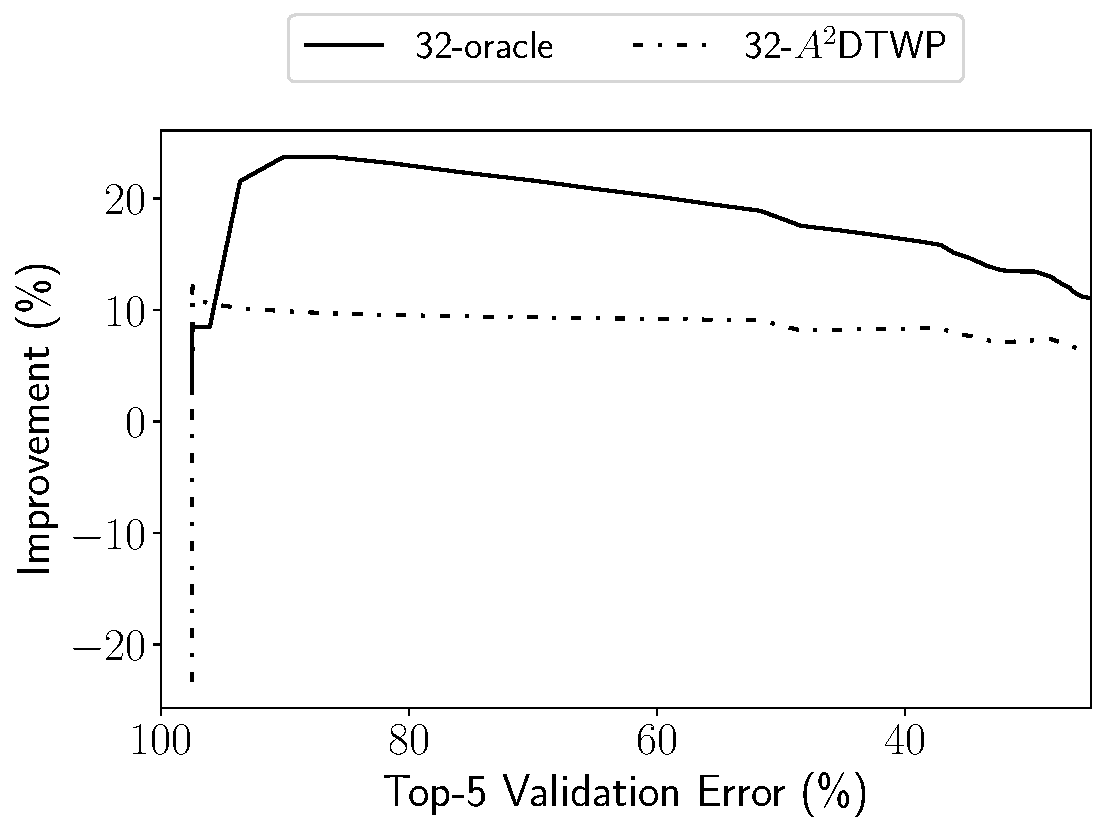
\includegraphics[scale=0.24]{figs/alex/small_3/alexnet_train_improvement_agg_top5_32-baseline.pdf}
%            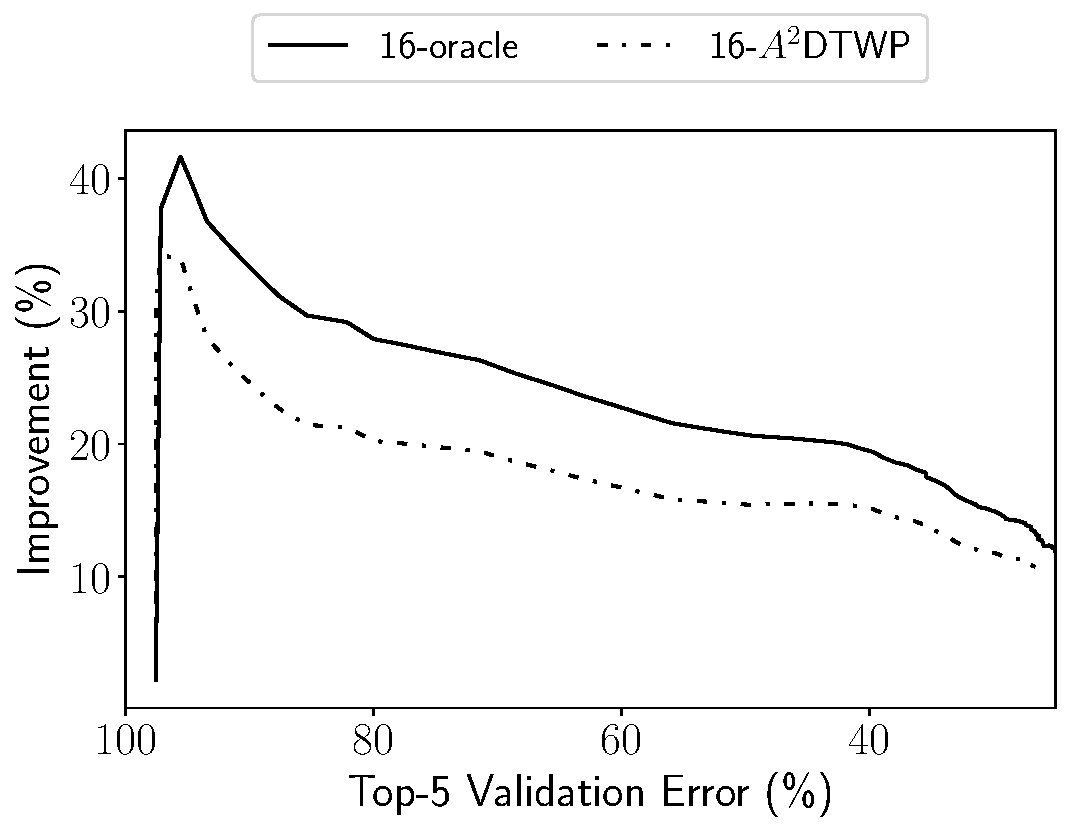
\includegraphics[scale=0.24]{figs/alex/small_3/alexnet_train_improvement_agg_top5_16-baseline.pdf}
%        }
%    \vspace{-0.4cm}
%    \caption{Results on Alexnet with two batch sizes: 32 and 16. The left
%    two figures show the top-5 validation error evolution of
%    \textit{baseline}, \textit{oracle} and \textit{$A^2$DTWP}.
%    The right two figures provide information on the performance improvement of
%    \textit{oracle} and \textit{$A^2$DTWP} against \textit{baseline}
%    during the training process. Experiments run on the x86 system.
%    \vspace{-0.5cm}
%    }
%        \label{alex_improv}
%\end{figure*}

\begin{figure*}[!bhtp]
    \hbox{%\hspace{7.0mm}
        \centerline{
            \includegraphics[scale=0.450]{figs/alex/small_3/alexnet_validation_top5_32-$A^2$DtWp.pdf}
            \includegraphics[scale=0.450]{figs/alex/small_3/alexnet_validation_top5_16-$A^2$DtWp.pdf}
        }
    }
    \hbox{%\hspace{7.0mm}
        \centerline{
            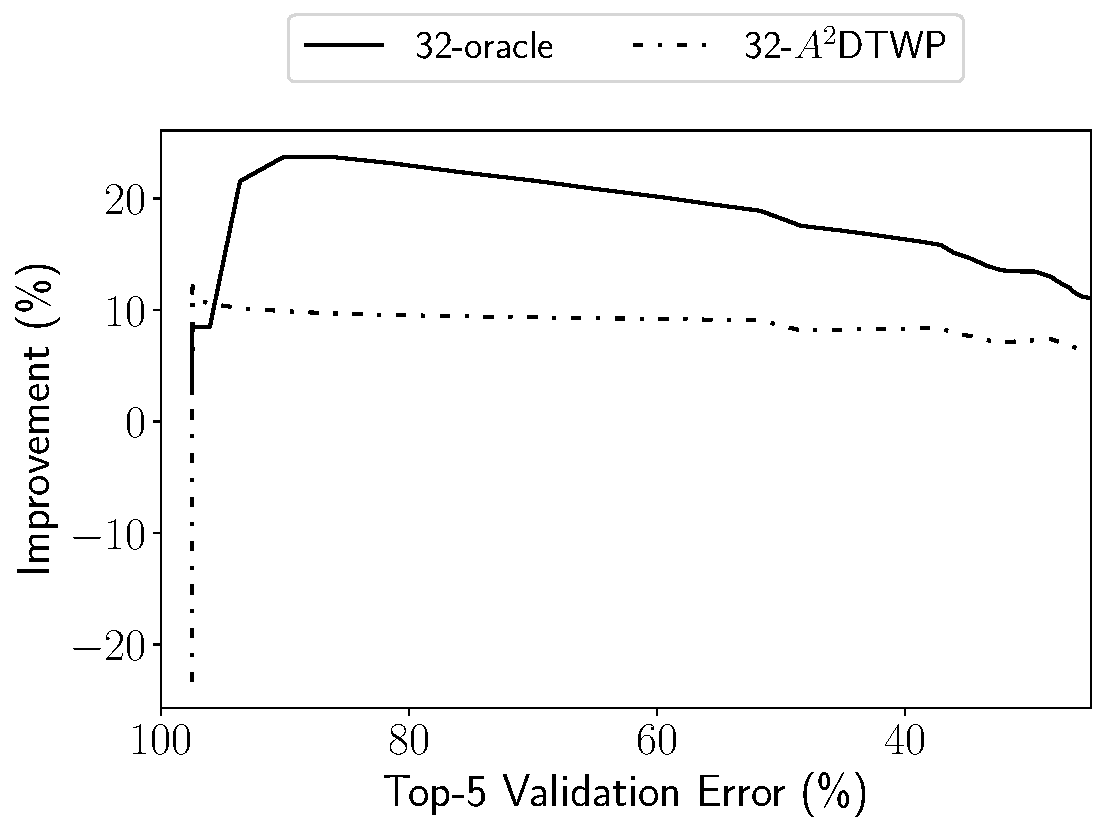
\includegraphics[scale=0.450]{figs/alex/small_3/alexnet_train_improvement_agg_top5_32-baseline.pdf}
            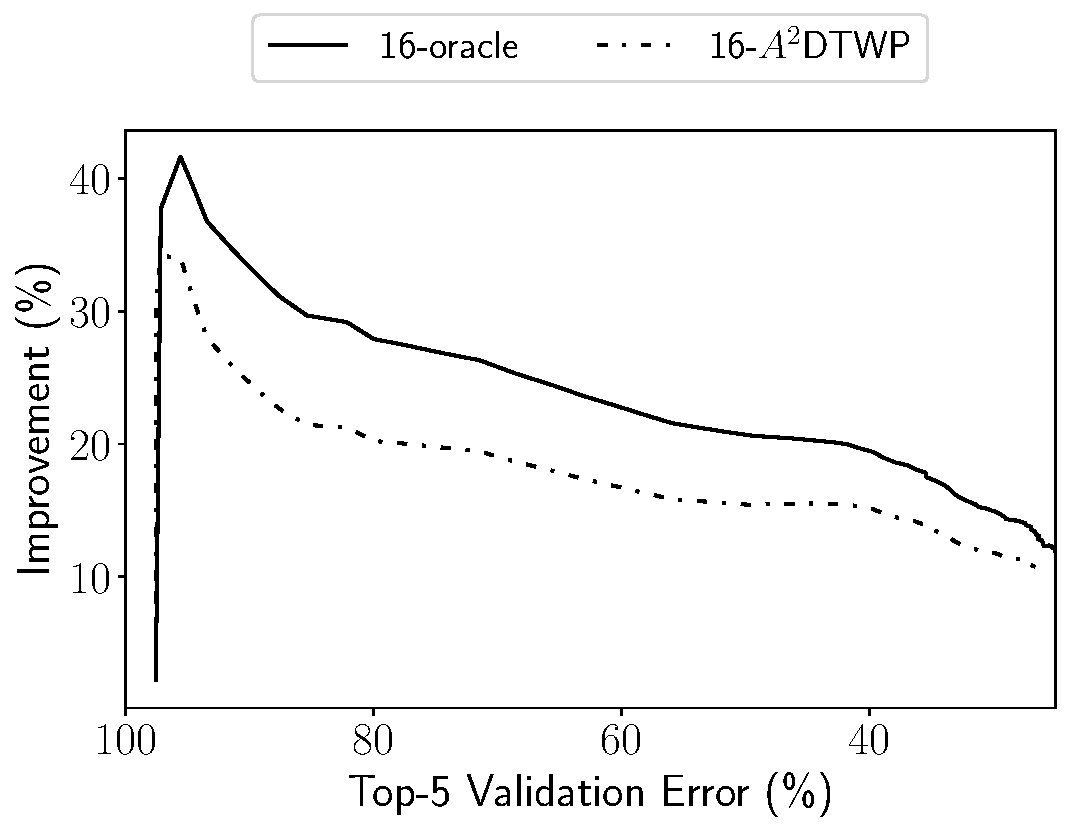
\includegraphics[scale=0.450]{figs/alex/small_3/alexnet_train_improvement_agg_top5_16-baseline.pdf}
        }
    }
    \caption{Alexnet training considering 32 and 16 batch sizes. The 
    two upper plots show the top-5 validation error evolution of
    \textit{baseline}, \textit{oracle} and \textit{$A^2$DTWP}.
    The two bottom plots provide information on the performance improvement of
    \textit{oracle} and \textit{$A^2$DTWP} against \textit{baseline}
    during the training process. Experiments run on the x86 system.
    %\vspace{-0.5cm}
    }
        \label{alex_improv}
\end{figure*}



\section{Evaluation}
\label{sec:evalutation}
In this section we evaluate the capacity of the AWP algorithm and the ADT procedure to accelerate DNNs training. 
We show how our proposals are able to accelerate the training phase of relevant DNN models without reducing the accuracy of the network. 
%to classify large image data sets. 

\subsection{Methodology}
\label{sec:evaluation1}

%\begin{figure*}[!bhtp]
%    \vspace{0.1cm}
%    \centerline{
%        \includegraphics[scale=0.24]{figs/vgg/small_3/vgg_validation_top5_64-$A^2$DtWp.pdf}
%        \includegraphics[scale=0.24]{figs/vgg/small_3/vgg_validation_top5_32-$A^2$DtWp.pdf}
%        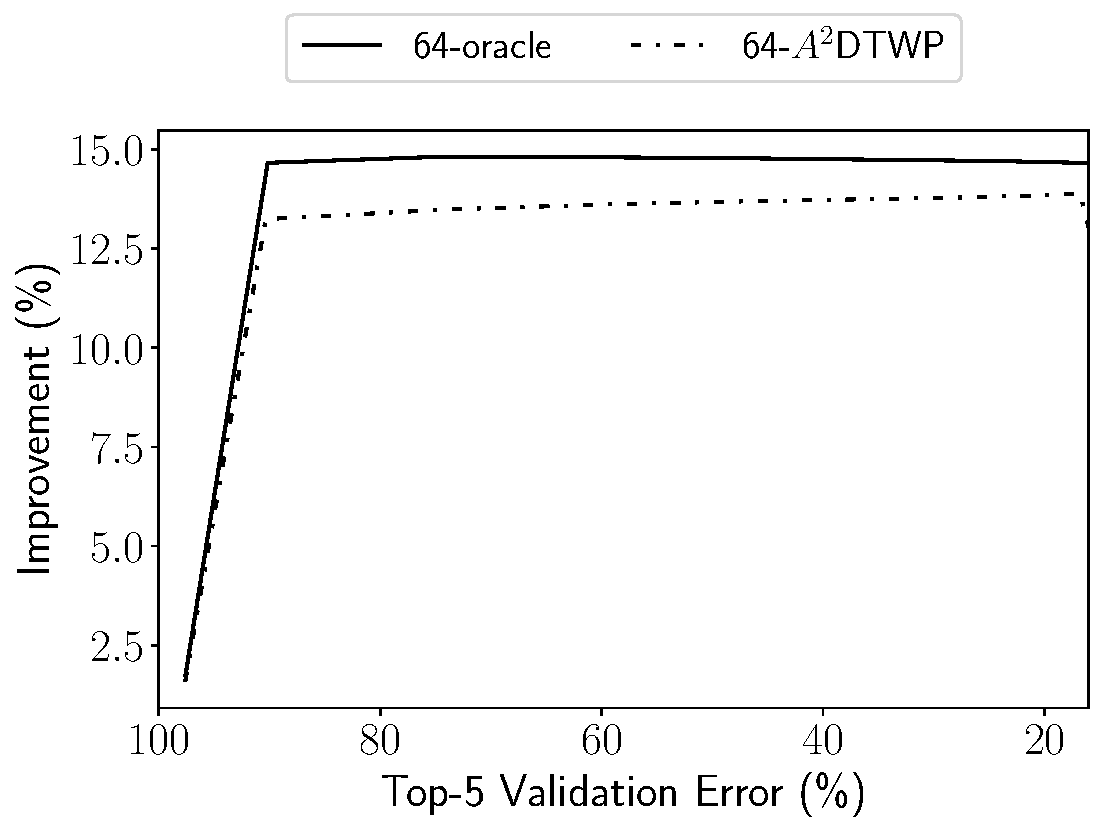
\includegraphics[scale=0.24]{figs/vgg/small_3/vgg_train_improvement_agg_top5_64-baseline.pdf}
%        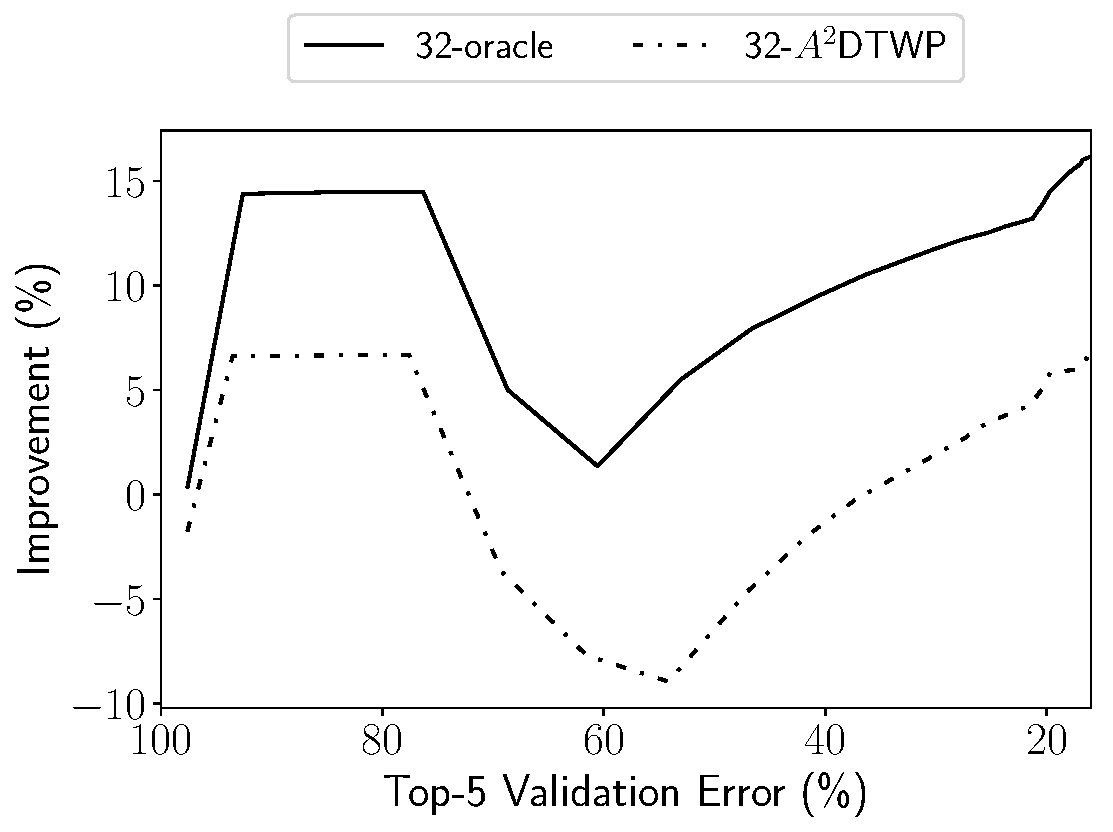
\includegraphics[scale=0.24]{figs/vgg/small_3/vgg_train_improvement_agg_top5_32-baseline.pdf}
%    }
%    \vspace{-0.4cm}
%    \caption{Results on VGG with two batch sizes: 64 and 32. The left
%    two figures show the top-5 validation error evolution of
%    \textit{baseline}, \textit{oracle} and \textit{$A^2$DTWP}.
%    The right two figures provide information on the performance improvement of
%    \textit{oracle} and \textit{$A^2$DTWP} against \textit{baseline} during the
%    training process. Experiments run on the x86 system.
%    %\rephrased{Figures upgraded from using continuous lines to using points}
%    }
%        \label{vgg_improv}
%    %\vspace{-0.5cm}
%\end{figure*}

\begin{figure*}[!bhtp]
    \hbox{%\hspace{7.0mm}
        \centerline{
            \includegraphics[scale=0.450]{figs/vgg/small_3/vgg_validation_top5_64-$A^2$DtWp.pdf}
            \includegraphics[scale=0.450]{figs/vgg/small_3/vgg_validation_top5_32-$A^2$DtWp.pdf}
        }
    }
    \hbox{%\hspace{7.0mm}
        \centerline{
            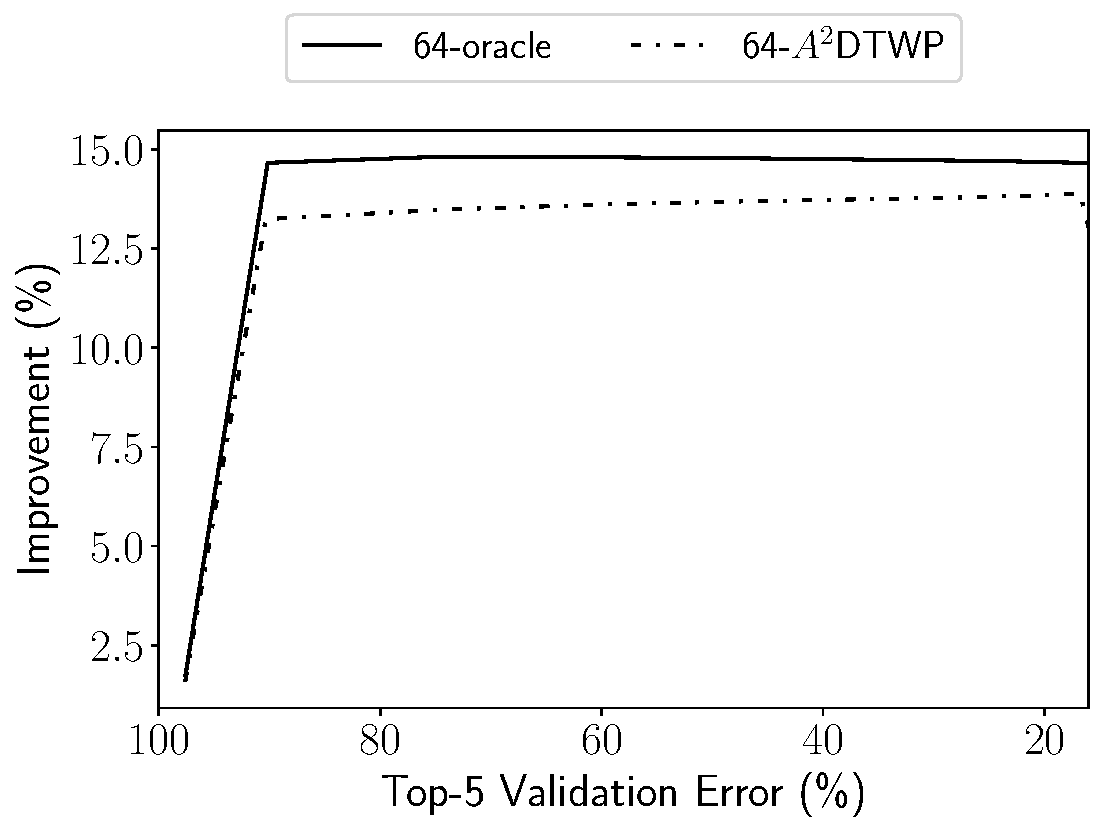
\includegraphics[scale=0.450]{figs/vgg/small_3/vgg_train_improvement_agg_top5_64-baseline.pdf}
            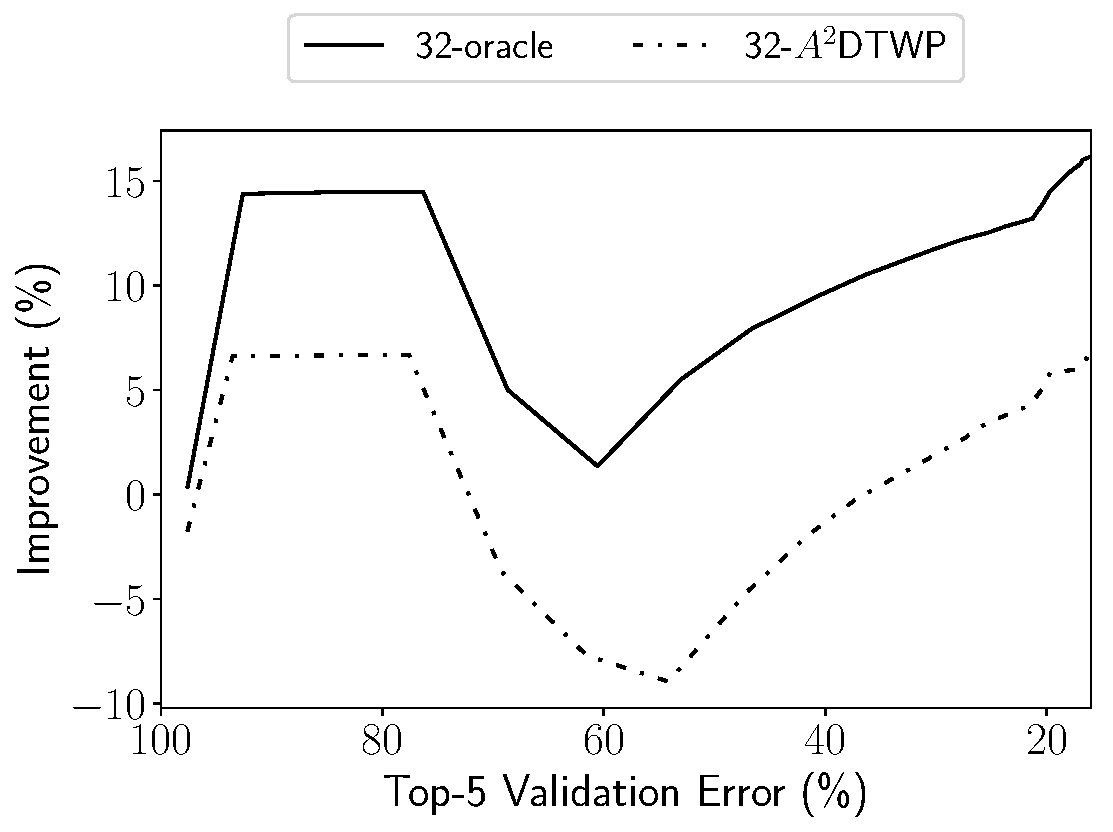
\includegraphics[scale=0.450]{figs/vgg/small_3/vgg_train_improvement_agg_top5_32-baseline.pdf}
        }
    }
    \caption{VGG training considering 64 and 32 batch sizes. The 
    two upper plots show the top-5 validation error evolution of
    \textit{baseline}, \textit{oracle} and \textit{$A^2$DTWP}.
    The two bottom figures provide information on the performance improvement of
    \textit{oracle} and \textit{$A^2$DTWP} against \textit{baseline} during the
    training process. Experiments run on the x86 system.
    %\rephrased{Figures upgraded from using continuous lines to using points}
    }
    \label{vgg_improv}
    %\vspace{-0.5cm}
\end{figure*}

%We conduct a set of experiments on several batch sizes (16, 32, 64) for both Alexnet and VGG. 
Our experimental campaign considers batch sizes of 64, 32 and 16 for the Alexnet and VGG models and 128, 64 and 32 for the Resnet network.
For each model and batch size, the \emph{baseline} run uses the 32-bit Floating Point precision for the whole training. 
The data represention formats we consider to transfer weights from the CPU to the GPU are:
8-bit (1 bit for sign, 7 bits for exponent), 16-bit (1 bit for sign, 8 for exponent, 7 for mantissa), 24-bit (1 bit for sign, 8-bits for exponent and 15 bits for mantissa) and 32-bits (1 bit for sign, 8 bits for exponent and 23 bits for mantissa).
We train the network models with dynamic data representation by applying the AWP algorithm along with the ADT procedure.
We denote this approach combining ADT and AWP as \textit{$A^2$DTWP}.  
For each DNN and batch size, we select the data representation format that first 
reaches the 35\%, 25\% and 15\% accuracy thresholds for Resnet, Alexnet and VGG, respectively, and we 
denote this approach as \emph{oracle}.
For the case of the \emph{oracle} approach, data compression is done via ADT.
The closer \textit{$A^2$DTWP} is to \emph{oracle}, the better is the AWP algorithm in identifying the best data representation format.

During training we sample data in terms of elapse time and validation error every 4000 batches. 
The total number of training batches corresponding to the whole ImageNet200 dataset are 16020, 8010, 4005 and 2002 for batch sizes 16, 32, 64 and 128, respectively.
The values of $AWP$ parameters $T$, $INTERVAL$, and $N$ are determined in the following way:
In the case of $T$ we monitor the execution of several epochs until we observe a drop in the validation error. 
We then measure the average change, considering all layers, of weights' $l^2$-norm during this short monitoring period.
The obtained values of $T$ are $-5\times10^{-2}$, $-2\times10^{-3}$ and $-2\times10^{-5}$ for Alexnet, VGG and Resnet, respectively.
We set the $INTERVAL$ parameter to $4000$ for both AlexNet and VGG and $2000$ for Resnet. 
These values correspond to a single batch (for the ImageNet200 dataset and batch sizes 64 and 128) and avoid premature precision switching due to numerical fluctuations.  
We set $N$ to $8$ since the smallest granularity of our approach is 1 byte.
AWP initially applies 8-bit precision to all layers.
We use ImageNet200 in Sections~\ref{sec:alexnet}, ~\ref{sec:VGG}, ~\ref{sec:Resnet}, ~\ref{sec:Average}, and ~\ref{sec:performance}.
Section~\ref{sec:ImageNet1000} uses ImageNet1000.

\subsection{Evaluation on Alexnet}
\label{sec:alexnet}
The evaluation considering the Alexnet model on the x86 system is shown in  
Figure~\ref{alex_improv}, which plots detailed results considering batch sizes of 
32 and 16, and Figure~\ref{fig:all}, which shows the total execution time of the 
\textit{oracle} and \textit{$A^2$DTWP} policies normalized to the \textit{baseline} 
for the 64, 32 and 16 batch sizes on both the x86 and the POWER systems.
The two top plots of Figure~\ref{alex_improv} depict how the validation error of the 
\textit{baseline}, \textit{oracle}, and \textit{$A^2$DTWP} policies evolves 
over time for the 32 and the 16 batch sizes until the 25\% accuracy is reached.
The two bottom plots provide information regarding the performance 
improvement of both \textit{oracle} and \textit{$A^2$DTWP} over the 
32-bit \textit{baseline} with regard to a certain validation error. 
Such performance improvement is computed by looking at the time required by the 
\textit{oracle} and \textit{$A^2$DTWP} techniques to reach a certain validation error with respect to the \textit{baseline}.

It can be observed in the upper left-hand side plot of Figure~\ref{alex_improv} how 
the \textit{oracle} and the \textit{$A^2$DTWP} approaches are 10.82\% and 6.61\% faster than the baseline, respectively, to reach the 25\% top-5 validation error when using a 32 batch size.
The upper right-hand side plot shows results considering a 16 batch size. 
The improvements achieved by the 
\textit{oracle} and \textit{$A^2$DTWP} approaches are 11.52\% and 10.66\%, respectively.
This demonstrates 
the efficiency of the ADT procedure in compressing and decompressing the network weights without undermining the performance benefits obtained from sending less data
from the CPU device to the GPU.
It also demonstrates the capacity of AWP to quickly identify the best data representation format per layer.

The two bottom plots of Figure~\ref{alex_improv} provide information on 
performance improvement of \textit{oracle} and \textit{$A^2$DTWP} over the \textit{baseline} during the training process.
%One of the right-hand side plots of Figure~\ref{alex_improv} shows results when considering the 32 batch size.
For the 32 batch size, \textit{oracle} reaches a peak improvement of 24.11\% when the 90\%  
validation error is reached and steadily declines from that point although it keeps a significant 
improvement of 10.82\% over the \textit{baseline} once the 25\% top-5 validation error is reached. 
\textit{$A^2$DTWP} falls in-between the \textit{baseline} and the \textit{oracle}  
and keeps its improvement above 7.03\% until it reaches the 27\% top-5 validation error.
Once it reaches the 25\% validation error \textit{$A^2$DTWP} is 6.51\% faster than the \textit{baseline}.
In conclusion, the \textit{$A^2$DTWP} policy is able to provide performance 
improvements that are close to the ones achieved by the best possible accuracy.
%while the \textit{best} reaches 9.39\% at 25\% validation error.
For the 16 batch size, the performance benefits of the 
\textit{oracle} policy reach a 41.64\% peak at the 94\% validation error point.
The \textit{$A^2$DTWP} policy reaches its maximum performance benefit, 34.21\%, when the validation error is 97\%.
At the 25\% validation error point, the \textit{oracle} and the 
\textit{$A^2$DTWP} policies reach 13.00\% and 10.75\% performance improvement, respectively.
Overall, results considering the Alexnet network for batch sizes 
32 and 16 confirm that \textit{$A^2$DTWP}, which combines both the 
AWP algorithm and the ADT procedure, successfully delivers very similar 
performance benefits to the best possible accuracy.

Figure~\ref{fig:all} shows the normalized execution time of the \textit{oracle} 
and \textit{$A^2$DTWP} policies with respect to the 32-bit FP \textit{baseline} on the x86 and the POWER systems. 
The top chart reports performance improvements of 10.75\%, 6.51\%, and 0.59\% for batch sizes 16, 32 and 64 in
the case of Alexnet runnig on the x86 system.  
For the 64 batch size, the marginal gains of \textit{$A^2$DTWP} over the \textit{baseline} are due the poor performance of the 8-bits format employed by \textit{$A^2$DTWP} at the beginning of the training process.
This format does not contribute to reduce the validation error for the 64 batch case, which makes the \textit{$A^2$DTWP} policy to fall behind the \textit{baseline} at the very beginning of the training process.  
Although \textit{$A^2$DTWP} eventually increases its accuracy and surpases the \textit{baseline}, it does not provide the same significant performance gains for Alexnet as the ones observed for batch sizes 16 and 32.

\textit{$A^2$DTWP} performance improvements on the POWER system in the case of 
Alexnet are 18.61\%, 14.25\% and 10.01\% with respect to the \textit{baseline} for batch sizes 16, 32 and 64, respectively.  
The POWER system achieves larger performance improvements than x86 since the 
Bitpack procedure can be further parallelized over the 40 cores of the POWER9 
multicore chips than the 16 cores available in the Haswell multicore devices of the x86 system. 
This mitigates the costs of weigths' compression and thus provides larger performance improvements. 

\subsection{Evaluation on VGG}
\label{sec:VGG}

Figure~\ref{vgg_improv} shows results for batch sizes 64 and 32 when using the 
VGG architecture on the x86 system. 
The upper figures display the temporal evolution of the validation error until the 15\% top-5 validation error is reached.
Like in Alexnet, both the \textit{$A^2$DTWP} and the \textit{oracle} policies outperform the \textit{baseline}.
In the case of batch size 64, both \textit{oracle} and \textit{$A^2$DTWP} 
display a similar evolution in terms of validation error, which translates to 
very close performance improvement over the baseline. 
They maintain an overall improvement of over 13.00\% against the \textit{baseline} 
during most of their training. The \textit{$A^2$DTWP} technique outperforms the baseline by 
12.88\% when reaches 15\% of top-5 validation error while the 
\textit{oracle} policy achieves the same improvement.
For batch size 32 the final improvement achieved by \textit{$A^2$DTWP} over the baseline is 5.02\%.
This improvement is not as large as the one achived for the 64 batch size since the AWP algorithm does not identify a numerical precision able to beat the \textit{baseline} until the 57\% validation error is reached, as it can be seen in the bottom right hand side plot of Figure~\ref{vgg_improv}. 
%Despite this issue, \textit{$A^2$DTWP} still achieves a remarkable performance improvement of {\bf XX\%} over the baseline.

Figure~\ref{fig:all} shows the normalized execution time of \textit{$A^2$DTWP} 
and \textit{oracle} with respect to the \textit{baseline} for VGG considering 
batch sizes of 16, 32 and 64 on the x86 and POWER systems.
When applied to the VGG model on the x86 system, \textit{$A^2$DTWP} outperforms the 32-bit Floating Point \textit{baseline} by 12.88\%, 5.02\% and 7.31\% for batch sizes 64, 32 and 16, respectively.
Despite the already described issues suffered by the \textit{$A^2$DTWP} technique when applied to the 32 batch size, this approach achieves very remarkable performance improvements over the baseline in all considered scenarios. 

The performance improvements observed when trying VGG on the POWER system are even higher.
\textit{$A^2$DTWP} outperforms the \textit{baseline} by 28.21\%, 20.19\% and 11.13\% when using the 16, 32 and 64 batch sizes, respectively.
The performance improvement achieved on the POWER system are larger than the ones observed for x86 since the Bitpack procedure can be parallelized over 40 cores when running on the POWER system.
We observe the same behavior for Alexnet, as Section~\ref{sec:alexnet} indicates.

\subsection{Evaluation on Resnet}
\label{sec:Resnet}
We display the normalized execution time of the \textit{$A^2$DTWP} and the \textit{oracle} policies when applied to the Resnet model using batch sizes of 128, 64 and 32 in Figure~\ref{fig:all}.
In the case of Resnet we do not show detailed plots describing the evolution of 
the validation error during training because its behavior is very close to some previously displayed scenarios like VGG.
On the x86 system, \textit{$A^2$DTWP} beats the 32-bit Floating Point baseline by 4.94\%, 4.39\% and 3.11\% for batch sizes of 128, 64 and 32, respectively, once a top-5 validation error of 30\% is reached.
The relatively low performance improvement achieved in the case of 32 batch size is due to a late identification of a competitive numerical precision, as it happens in the case of VGG and batch size 32.

The performance gains on the POWER system display a similar trend as the ones achieved on x86. 
While they show the same low improvement for the 32 batch size, 2.12\%, \textit{$A^2$DTWP} achieves 6.92\% and 11.54\% performance gains for batch sizes 64 and 128, respectively.
\textit{$A^2$DTWP} achieves the largest performance improvement with respect to the 32-bit \textit{baseline} when run on the POWER system due to the reasons described in Sections~\ref{sec:alexnet} and~\ref{sec:VGG}.

\subsection{Average Performance Improvement}
\label{sec:Average}
The average performance improvement of \textit{$A^2$DTWP} over the 
\textit{baseline} considering the Alexnet, VGG and Resnet models reach 6.18\% and 11.91\% on the x86 and the POWER systems, respectively. 
As we explain in previous sections, \textit{$A^2$DTWP} obtains larger improvements on the POWER system than on  
x86 since the ADT procedure can be further parallelized over the 40 cores of the POWER9 multicore devices.
In contrast, the two Haswell devices of the x86 system offer just 16 cores for ADT.

The combination of the AWP algorithm and the ADT procedure properly adapts the precision of each network layer and compresses the corresponding weigths with a minimal overhead.
The large performance improvement obtained while training deep networks on two high-end computing systems demonstrate the effectiveness of \textit{$A^2$DTWP}.

\begin{figure}%[!bhtp]
    \centerline{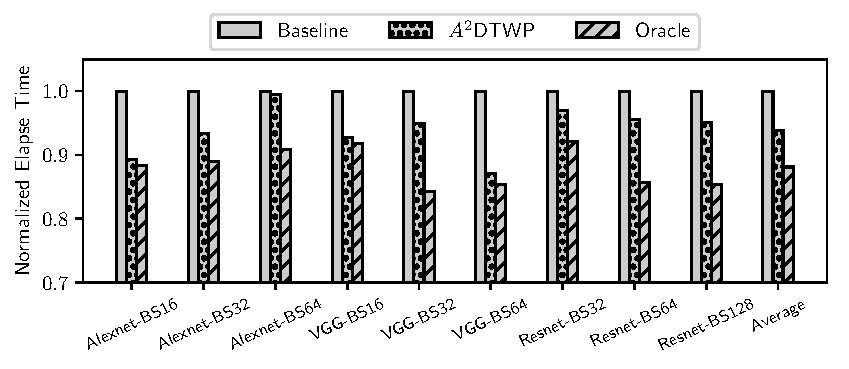
\includegraphics[scale=0.65]{figs/all_bars.pdf}}
    \vspace{-0.2cm}
    \centerline{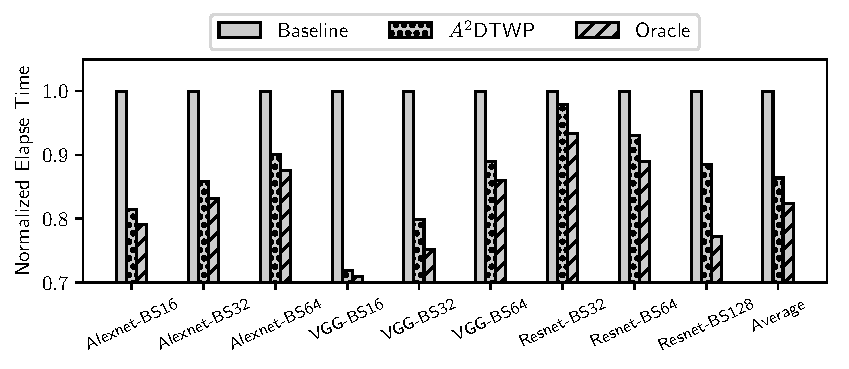
\includegraphics[scale=0.65]{figs/all_bars_p9.pdf}}
    \vspace{-0.5cm}
    \caption{Normalized execution times of the \textit{$A^2$DTWP} and the \textit{oracle} policies with respect to the baseline. 
Results obtained on the x86 system appear in the upper plot while the evalution on the POWER system appears at the bottom.} 
    %\textcolor{cyan}{Average: 
    %$A^2$DtWp 0.938, oracle 0.881}}
    \label{fig:all}
\end{figure}

\subsection{$A^2DTWP$ Performance Profile}
\label{sec:performance}
This section provides a detailed performance profile describing the effects of 
applying $A^2DTWP$ when training the VGG network model with batch size 64 on the x86 and POWER systems described in section~\ref{sec:platform}.
To highlight these effects we also show a performance profile of applying 32-bit 
Floating Point format during training.
The main kernels involved in the training process and their corresponding average execution time in milliseconds are shown in Tables ~\ref{table:performance} and~\ref{table:performance_p9}.
Each kernel can be invoked multiple times by different network layers and it can be overlapped with other operations while processing a batch.
Tables~\ref{table:performance} and~\ref{table:performance_p9} display for all kernels the average execution time of their occurrences within a batch when run on the x96 and the POWER systems, respectively.
%In order to to demonstrate the performance of our $A^2DtWp$ approach, we 
%dissect a typical batch in VGG BS32 (the baseline and the $A^2DtWp$ when 
%ROUNTO=16) into the operations involved and their elapse time in the 
%Table~\ref{table:performance}. 
%Each operation can be invoked multiple times on different layers during a batch 
%and can be overlapped with other operations so we take the average value of all 
%the occurrences in a batch. 
%Nevertheless, it gives an insight look into the efficiency of our approach.

Results appearing in Table~\ref{table:performance} show how time spent transferring 
data from the CPU to the GPU accelerators when applying $A^2DTWP$ on the x86 system, 52.27 ms, 
is significantly smaller than the cost of performing the same operation when using the 32-bit configuration, 153.93 ms. 
This constitutes a 2.94x execution time reduction that compensates the cost of the operations involved in the ADT routine, Bitpack and
Bitunpack, and in the AWP algorithm, the $l^2$-norm computation.
On POWER we observe a similar reduction of 3.20x in the time spent transferring
data from the CPU to the GPUs when applying $A^2DTWP$.
These reductions in terms of CPU to GPU data transfer time are due to a close to 3x reduction in terms of weights size enabled by $A^2DTWP$.
The average execution time of operations where the $A^2DTWP$ technique plays no role remains very similar for the 32-bit Floating Point baseline and $A^2DTWP$ in both systems, as expected.
Tables~\ref{table:performance} and~\ref{table:performance_p9} indicate that performance gains achieved by $A^2DTWP$ are due to data motion reductions, which validates the usefulness of $A^2DTWP$.

Tables~\ref{table:performance} and~\ref{table:performance_p9} also display the overhead associated with AWP and ADT in terms of milliseconds.
The AWP algorithm spends most of its runtime computing the $l^2$-norm of the weights, which takes a total of 3.88 ms within a batch on the x86 system. 
On POWER, the cost of computing the $l^2$-norm of the weights is 0.93 ms.
The other operations carried out by AWP have a negligible overhead.
The two fundamental procedures of ADT are the Bitpack and Bitunpack routines, which take 19.71 and 4.51 ms to run within a single batch on the x86 system.
For the case of POWER, Bitpack and Bitunpack take 10.51 and 1.11 ms, respectively.
Overall, measurements displayed at Table~\ref{table:performance} indicate that AWP and ADT constitute 1.05\% and 6.60\% of the total batch execution time, respectively, on x86.
On the POWER system, AWP and ADT constitute 0.54\% and 6.82\% of the total batch execution time according to Table~\ref{table:performance_p9}. 
Figures ~\ref{alex_improv}, ~\ref{vgg_improv} and ~\ref{fig:all} account for this overhead in the results they display.

\begin{table}
    \caption{Performance profiles of both the $A^2DTWP$ and the 32-bit Floating 
    Point approaches expressed in milliseconds on the x86 system. 
    We consider the VGG network model with batch size 64.} 
    \vspace{-0.35cm}
    \centering
    \begin{tabular}{|P{4.2cm}|P{1.5cm}|P{1.5cm}|}
    \hline
    %\rowcolor{LightCyan}
    & \textbf{32-bit FP} & $\mathbf{A^2DTWP}$\\
    \hline
    %\rowcolor{LightCyan}
    Data Transfer CPU$\rightarrow$GPU& 153.93 & 52.27 \\
    \hline
    %\rowcolor{LightCyan}
    Data Transfer GPU$\rightarrow$CPU& 68.51 & 73.55 \\
    \hline
    %\rowcolor{LightCyan}
    Convolution & 128.72 & 126.13\\
    \hline
    %\rowcolor{LightCyan}
    Fully-connected & 33.51 & 34.17 \\
    \hline
    %\rowcolor{LightCyan}
    Gradient update & 54.39 & 52.86\\
    \hline
    %\rowcolor{LightCyan}
    AWP ($l^2$-norm) & N/A & 3.88 \\
    \hline
    %\rowcolor{LightCyan}
    ADT (Bitpack) & N/A & 19.71 \\
    \hline
    %\rowcolor{LightCyan}
    ADT (Bitunpack) & N/A & 4.51 \\
    \hline
    \end{tabular}
    \label{table:performance}
\end{table}

\begin{table}
    \caption{Performance profiles of both the $A^2DTWP$ and the 32-bit Floating 
    Point approaches expressed in milliseconds on the POWER system. 
    We consider the VGG network model with batch size 64.} 
    \vspace{-0.35cm}
    \centering
    \begin{tabular}{|P{4.2cm}|P{1.5cm}|P{1.5cm}|}
    \hline
    & \textbf{32-bit FP} & $\mathbf{A^2DTWP}$ \\
    \hline
    Data Transfer CPU$\rightarrow$GPU& 39.12 & 12.21 \\
    \hline
    Data Transfer GPU$\rightarrow$CPU& 17.34 & 17.87 \\
    \hline
    Convolution & 69.78 & 71.21\\
    \hline
    Fully-connected & 12.66 & 13.51 \\
    \hline
    Gradient update & 41.29 & 42.98\\
    \hline
    AWP ($l^2$-norm) & N/A & 0.93 \\
    \hline
    ADT (Bitpack) & N/A & 10.51 \\
    %Bitpack & N/A & 10.51 \\
    \hline
    ADT (Bitunpack) & N/A & 1.11 \\
    %Bitunpack & N/A & 1.11 \\
    \hline
    \end{tabular}
    \label{table:performance_p9}
\end{table}

\subsection{Experiments with ImageNet1000}
\label{sec:ImageNet1000}
%We run experiments considering ImageNet1000 to confirm they display the same trends as results shown in Sections~\ref{sec:alexnet}, ~\ref{sec:VGG}, ~\ref{sec:Resnet}, ~\ref{sec:Average}, and ~\ref{sec:performance}, which consider ImageNet200.
We run experiments considering ImageNet1000 to confirm they display the same trends as executions with ImageNet200. 
Network parameters are the same as the ones described in Section~\ref{sec:setup}.
$AWP$ parameters are the ones described in Section~\ref{sec:evaluation1}.
The experimental setup of the evaluation considering ImageNet1000 is the same as the one we use for ImageNet200.
We consider batch sizes that produce the fastest 32-bit FP training for each one of the network models: 64, 64, and 128 for Alexnet, VGG and Resnet, respectively.


Figure~\ref{fig:ImageNet1000} displays results corresponding to the experimental campaign with ImageNet1000 on the x86 system.
In the x-axis we display different epoch counts for each one of the three models: 4, 8, 12, 16, and 20 epochs for Alexnet; 2, 4, 6, and 8 for VGG; and 4, 8, 12, and 16 epochs for Resnet.
The y-axis displays the normalized elapsed time of \textit{$A^2$DTWP} with respect to the the 32-bit Floating Point \textit{baseline} per each model and epoch count.
For the case of Alexnet with batch size 64, \textit{$A^2$DTWP} is slightly faster than the \textit{baseline} as it displays a normalized execution time of 0.995, 0.992, 0.992, 0.996, and 0.990 after 4, 8, 12, 16 and 20 epochs, respectively.
Figure~\ref{fig:all} also reports small gains for the case of Alexnet with batch size 64, which confirms that experiments with ImageNet1000 show very similar trends as the evaluation with ImageNet200.
When applying \textit{$A^2$DTWP} to VGG with 64 batch size, it displays a normalized execution time of 0.907, 0.920, 0.936, and 0.932 with respect to the \textit{baseline} after running 2, 4, 6 and 8 training epochs, respectively.
For the Resnet example, we observe normalized execution times of 0.765, 0.770, 0.778, and 0.777 for \textit{$A^2$DTWP} after 4, 8, 12, and 16 training epochs, respectively,
which constitutes a significant performance improvement.

\begin{figure}%[!bhtp]
    \centerline{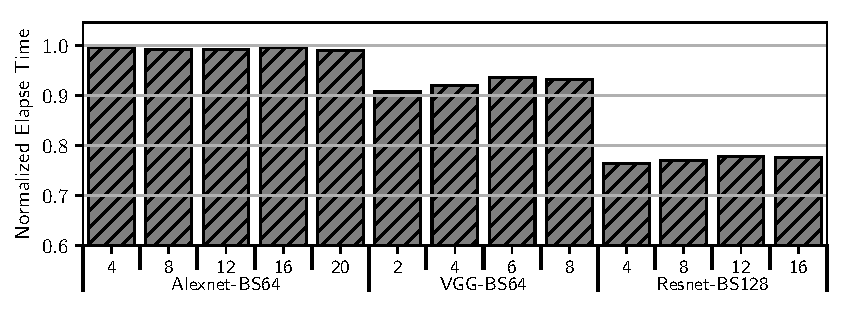
\includegraphics[scale=0.65]{figs/imagenet-1k-3net.pdf}}
    \caption{Normalized execution time of \textit{$A^2$DTWP} with respect to \textit{baseline} considering the Imagenet1000 data set. Training for Alexnet, VGG and Resnet considers up to 20, 8, and 16 epochs, respectively.}
    %\vspace{-0.5cm}
    \label{fig:ImageNet1000}
\end{figure}

In terms of validation error, both \textit{$A^2$DTWP} and \textit{baseline} display very similar top-5 values at the end of each epoch.
%For example, for the case of VGG, the Floating Point 32-bit \textit{baseline} approach displays validation errors of 88.04\%, 64.02\%, 56.46\%, and 46.18\% after 2, 4, 6, and 8 training epochs. 
%\textit{$A^2$DTWP} achieves validation errors of 89.97\%, 67.12\%, 55.99\%, and 46.89\% for the same epoch counts.
For example, for the case of VGG, the Floating Point 32-bit \textit{baseline} approach displays a validation error of 88.04\% after 2 training epochs while \textit{$A^2$DTWP} achieves a validation error of 89.97\% for the same epoch count, that is, an absolute difference of 1.93\%.
After 4, 6, and 8 training epochs absolute distances of top-5 validation errors between \textit{$A^2$DTWP} and \textit{baseline} are 3.09\%, 0.47\%, and 0.71\%, respectively.
Top-5 validation error keeps decreasing in an analogous way for both \textit{baseline} and \textit{$A^2$DTWP} as training goes over more epochs, although \textit{$A^2$DTWP} is significantly faster.
Our evaluation indicates that \textit{$A^2$DTWP} can effectively accelerate training while achieving the same validation error as the 32-bit FP \textit{baseline} when considering ImageNet1000.

%\subsection{$A^2DTWP$ Data Movement Reduction}
%Table~\ref{table:transfer} shows the avergage data movement in MB between the CPU 
%host and GPUs at the beginning of each batch on the POWER system on three 
%particular networks, Alexnet-BS32, VGG-BS32 and Resnet-BS128. The $A^2DTWP$ 
%reduces the data movement by 19.38\%, 24.8\% and 15.94\% respectively.
%
%\begin{table}[H]
%    \caption{Average data transfer per batch on the POWER system (MB)}
%    \vspace{-0.35cm}
%    \centering
%    \begin{tabular}{|P{4.2cm}|P{1.5cm}|P{1.5cm}|}
%    \hline
%    & \textbf{32-bit FP} & $\mathbf{A^2DTWP}$\\
%    \hline
%    Alexnet-BS32 & 98.63 & 79.81 \\ %19.38
%    \hline
%    VGG-BS32 & 387.92 & 291.54 \\ %24.8
%    \hline
%    Resnet-BS128 & 69.05 & 58.07 \\ %15.94
%    \hline
%    \end{tabular}
%    \label{table:transfer}
%\end{table}


%\subsection{Analysis of Weights' Dynamic Range}
%\label{sec:histograms}
%This section describes the weights' dynamic range of VGG's 9th layer by showing its distribution of weights' values at different points of the training process. 
%Figure~\ref{fig:hist} plots four different distributions corresponding to 0\%, 50\%, 75\% and 100\%, respectively, of VGG's training process with the batch size parameter set to 64.
%These distributions are generated with the 32-bit floating point precision.
%We can see in Figure~\ref{fig:hist} how the initial distribution of weights is randomly generated. % over the interval $[-0.27;0.27]$.
%As training progresses there is an increasing amount of weights with values very close to $0$
%, which is a trend observed for most of the layers of the VGG, the Alexnet and the Resnet models.
%What explains the usefulness of our approach is the fact that during the initial stages of the training process weight's values are far from the final ones. 
%As training progresses, weights values become closer to their final ones and more accuracy is required to keep adjusting them.
%\begin{figure}%[!bhtp]
%    \centerline{
%        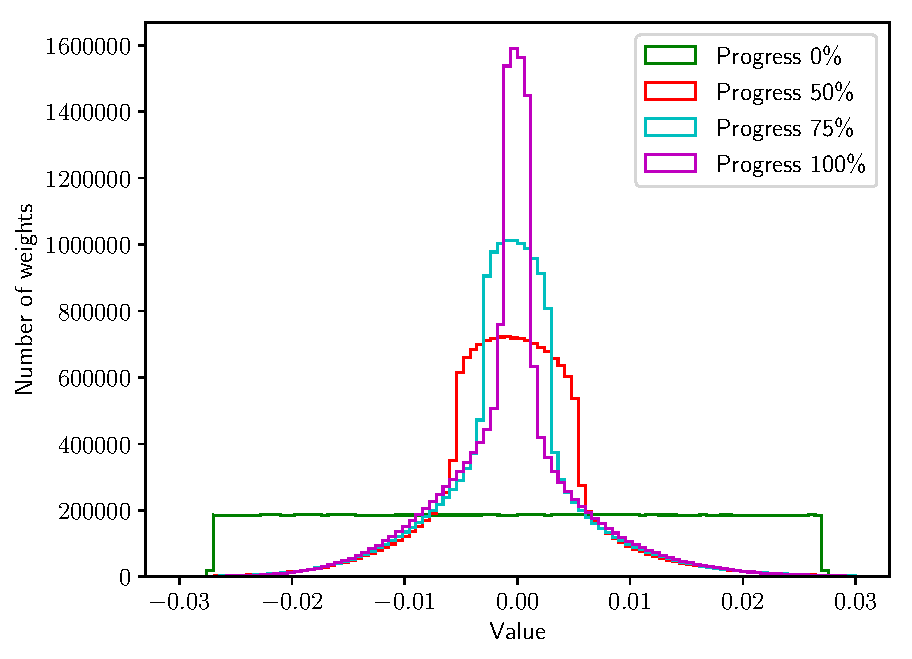
\includegraphics[scale=0.60]{figs/weights_9.pdf}
%    }
%    \vspace{-0.5cm}
%    \caption{Values' weights distribution considering the 9th layer of VGG with BS=64.} 
%    \label{fig:hist}
%    \vspace{-0.3cm}
%\end{figure}
